\chapter{Introduction}\label{chap:introduction}%
% Problem tanimi
% Neden cozmek istiyoruz
\section{Dictionaries}%
\label{sec:dictionaries}
Dictionary is a broad concept to define since lexicographers prepare them for various specific use cases.
For instance, bilingual dictionaries present words alongside their translations in the target language.
Domain specific dictionaries list technical terms that target people who are familiar with the terminology.
Yet, the term \emph{dictionary} on its own brings forth the monolingual type, sometimes known as descriptive, into consideration.
This type of dictionary presents words alongside their definitions following an alphabetical order~\cite{sterkenburg_practical_2003}.
Their primary intention is to inform the user about the words~\cite{uzun_modern_2005}.
Some words are polysemous, sharing the same spelling and having related, often derivative meanings.
These different senses are clarified through multiple definition entries.
On the other hand, homonymous words have distinct meanings while having identical spellings through coincidence.
They are often denoted using discrete blocks of descriptions.
Finally, the last lexical relation is the synonymity.
A word is synonymous to another if they share the same meaning but are not spelled alike.
The term that precede the entries are called \emph{headword} or \emph{lemma}.
Usually, lemmas are the form of a word without inflections or derivations.
The sense they convey is as comprehensive as possible, reducing the number of otherwise redundant entries that would be the derivatives of the unmarked form~\cite{ibrahim_usta_turkce_2006}.

% from dictionaries to multilingual web
Dictionaries take an immense amount of time and expertise to prepare.
We can list the examples after narrowing our scope down to the dictionaries that are still available to use today.
A survey by \textcite{uzun_1945ten_1999} notes that the first instalment of the modern Turkish dictionary, led by a team of experts, has taken over 6 years to prepare.
\textcite{kendall_forgotten_2011} talks about how Noah Webster, the writer of the \emph{An American Dictionary of the English Language} had to mortgage off his home in order to finish his project which took over 26 years.
Early lexicographers had invest tremendous amounts of time in order to collect enough material to prepare a collection of documents, also knows as a \emph{corpus}~\cite{uzun_1945ten_1999}.
This endeavour is necessary since a corpus is crucial to create the vocabulary of a language.
After the corpus is processed, lemmas are extracted and the resulting wordstock is called the \emph{lexicon}.

The internet radically changed the way researchers aggregate the data.
The advancements in digital storage technology allowed the data to be persistent.
Improvements in networking ensured that people can share the volume of it among themselves.
With the popularization of the social media, the internet generates everyday conversations at an unprecedented rate that researchers are using for natural language applications. % TODO any reference
Moreover,  efforts on open, collaborative, web based encyclopedias generate structured, multilingual data often used in machine translation and text categorization tasks. % TODO any reference
Once cumbersome task of corpus attainment is now akin to web crawling.
With the digitized data, it was only natural for dictionaries to go digital as well since it's generally acknowledged that they are no longer viable if they are not electronic~\cite{sterkenburg_practical_2003}.

% start wordnets
\section{WordNet}% not sold on having 'wordnet' as a section
\label{sec:wordnet}
WordNet was initially thought up as a semantic network, consisting of lexical nodes. % citation here?
Its primary purpose was to depict patterns among those nodes.
George Miller, the project lead, believed that the right semantic graph would make the definitions redundant.
A sense would be identifiable solely through its place on the graph and relationship with the other senses.
%Lesk identified the primary power of such a network as a browser.
A traditional dictionary is constrained to the rigid written format.
Once the seeked entry is reached, the flow of information stops.
The spelling and meaning information is gained but there is nowhere to go from there.
As seen in Figure~\ref{fig:example_run}, a query on WordNet leads to a network of semantically related concepts.
Over the years, WordNet evolved from a semantic network to a lexical database~\cite{fellbaum_wordnet_1998}.

In the context of dictionaries, we have emphasized lemmas and definitions.
Once again, lemmas are used to index the WordNet.
However, there is no need for them to be arranged alphabetically.
When a word is looked up on WordNet, the \emph{senses} that are represented by the term come up.
\ref{fig:example_run} shows the truncated result for the query word \enquote{run} .
The lookup string is the lemma while the results can list other lemmas alongside it or around it.
The set of lemmas that are given in one line
All the lemmas that are given with the sense can depict the sense can be denoted by any and all lemmas give.
The set of these synonyms is aptly named synset.
The elements of a synset share the same meaning, WordNet includes a definition, called a \emph{gloss} to go alongside them.
WordNet is built on relations between the senses.
One such relation is hyponymy
WordNet can show relationships like hyponymym, the hierarchy information for words that are subordinates of another.
For instance, an \emph{automobile} and a \emph{boat} are both subtypes of the broader term \emph{vehicle}.
Another relationship is called meronymym.
Part-whole relation, only possible with an electronic resource.
\textcite{fellbaum_semantic_1998} defines the correct terminology that we abide for the thesis; \enquote{As WordNet became synonymous with a particular kind of lexicon design, the proper name shed its capital letters and became a common designator for semantic networks of natural languages}.
Hence \emph{WordNet} refers to English Princeton WordNet, while wordnets created for other languages are not stylized.
\begin{figure*}[!hbp]
    \begin{center}
        {%
            \setlength{\fboxsep}{1pt}%
            \setlength{\fboxrule}{1pt}%
            \fbox{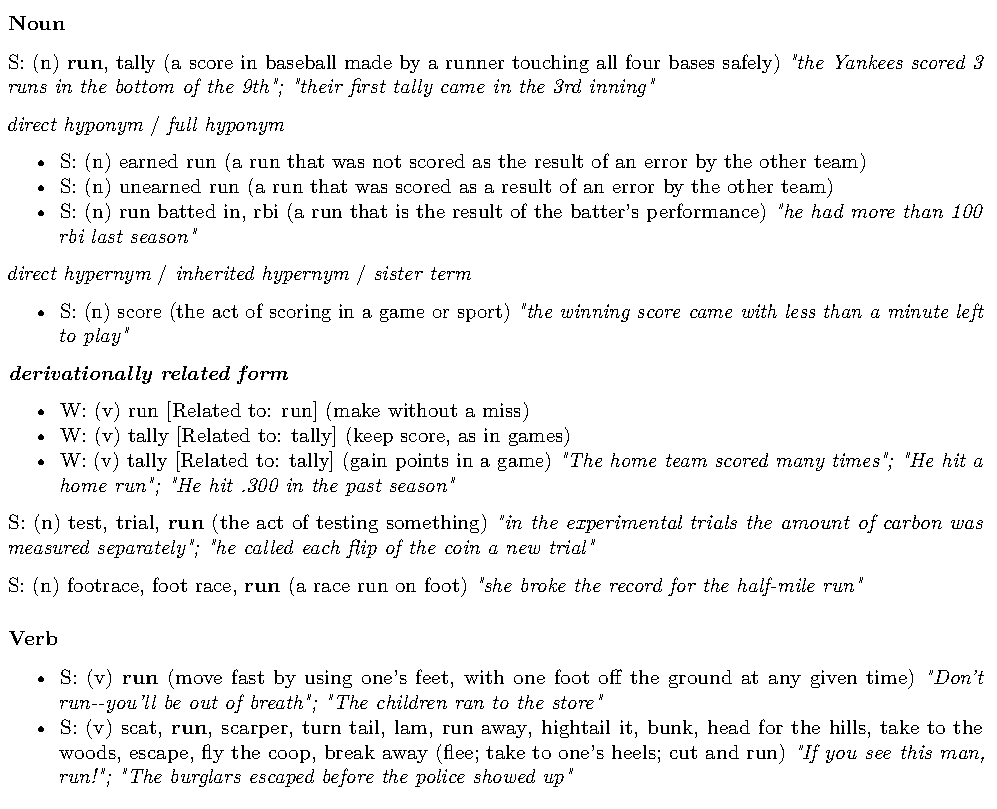
\includegraphics[page=1,width=\textwidth]{Figures/run_wordnet.pdf}}
        }%
    \caption{WordNet result for the query \enquote{run}, truncated for brevity.}\label{fig:example_run}
    \end{center}
\end{figure*}

\section{Multilingual Wordnets}%
\label{sec:multilingual_wordnets}
Authorities list more than 7000 living languages\footnote{\url{https://www.ethnologue.com/statistics}} with only 40\footnote{\url{https://w3techs.com/technologies/history_overview/content_language/}} of them having a sizeable presence on the internet.
Nevertheless, among this small fraction, English is the dominant language of the web.
Translation, information transfer from foreign languages is a valid way of enriching a language's corpora.
If a word for a sense does not have a match in target language, it is a good indication for the linguists of that language to look into their lexicons and maybe expand it~\cite{ibrahim_usta_turkce_2006}.
We should note that the languages of the wordnets used in the thesis are all present in the 40 languages that have a significant presence on the internet that we have mentioned before.
\textcite{sagot_building_2008} argues that linking wordnets leads to more research and there seems to be a vicious cycle between the available data for a language to form a lexicon and a corpus.
Further research in the area contributes to more languages having access to tools that will incorporate them into the literature.
English in not the centrepiece for most natural language processing research because it is the language that can store the most information or any other linguistic advantage.
It's the most abundant language on web.
Distributions like spaCy resorts to lemmatizations such as \emph{=PRON=} to denote pronouns in order to collapse the senses for \enquote{I} \enquote{you}, \enquote{them} etc.\@.
Whereas phrases like

% might be too cheesy
% The sense and the accompanying word for being the brother of someone's father or mother differs in Turkish.\footnote{\emph{Amca} for brother of the father and \emph{Dayı} for brother of the father.}
% Yet no distinction exists for English and senses collapse together in \emph{uncle}.
% \might be too cheesy

The work on wordnets for languages other than English has been under way since the early days of the predecessor.

Research has tackled the issue of lack of wordnets for languages besides English. %TODO reference

Yet, against %TODO how many?
senses in the English Princeton WordNet, the most comprehensive counterpart remain at ... % TODO how many
Coupled with the licensing issue which prevents scientific research from using some WordNets.
We have constrained this study to use only the freely available wordnets.
Open Multilingual WordNet~\cite{bond_survey_2012} presents wordnets from other languages with three crucial additions; % TODO the following sentence is plagiarism
They have normalized the data, aligned with English Princeton WordNet and they are all accessible from a single source.\footnote{\url{http://compling.hss.ntu.edu.sg/omw/}}
With alignment information at hand, we have a way to create a golden corpora that we assume to be perfectly aligned.
Among the 34 wordnets available on Open Multilingual WordNet, only 6 of them have gloss information available.
Given this thesis will only investigate the ability to map senses using definitions of the sense, we used the subset of Albanian~\cite{ruci_current_2008}, Bulgarian~\cite{simov_constructing_2010}, Greek~\cite{stamou_exploring_2004}, Italian~\cite{pianta_multiwordnet_2002}, Slovenian~\cite{fiser_slownet_2012} and Romanian~\cite{tufis_romanian_2008}.
Table~\ref{tab:summary_table} shows brief statistics about the wordnets.

\begin{table*}[!hbp]
    \begin{center}
        \caption{Summary of the Wordnets used.}\label{tab:summary_table}
        \begin{tabular}{llrr}
            \toprule%
            \textbf{Name of the Project} & \textbf{Language} & \textbf{Number of Definitions} & \textbf{Words Per Definition} \\
            \midrule%
            Albanet & Albanian & 4681 & 11.75 \\
            BulTreeBank WordNet & Bulgarian & 4959 & 12.71 \\
            % DanNet & Danish    & 784                   & 8.63                           \\
            Greek Wordnet & Greek & 18136 & 11.24 \\
            ItalWordnet & Italian & 12688 & 7.33 \\
            Romanian Wordnet & Romanian & 58754 & 9.98 \\
            SloWNet & Slovenian & 3144 & 12.68 \\
            \bottomrule %
        \end{tabular}
    \end{center}
\end{table*}

\section{Word Embeddings}%
\label{sec:word_embeddings}
James Somers puts down the modern dictionaries by saying \enquote{The definitions are these desiccated little husks of technocratic meaningese, as if a word were no more than its coordinates in semantic space.}~\cite{somers_youre_2014}.
From his perspective an an author, the efficient descriptions that are found in dictionaries might be a bother but we will build the thesis on the idea that we can represent words, senses using their dictionary definitions.
For research on languages other than English to benefit from the power of wordnet the languge should have copious data available to generate corpora.
However, traditional dictionaries are more commonly available and include definition information.

\section{Thesis Goals}%
\label{sec:thesis_goals}
In this thesis, our aim is to study the possibility of creating wordnets using dictionary alignment.
We will evaluate existing methods for their performance on cross-lingual document retrieval but our documents are dictionary definitions which are short, descriptive snippets of text.

\section{Thesis Outline}%
\label{sec:thesis_outline}
\texttt{Fill later\ldots}
